\chapter{Estado del arte}
\label{estado.arte}

\section{Impresoras 3D}
\label{arte_immpresoras}
En los últimos años ha tenido un gran auge las denominadas impresoras 3D. Máquinas capaces de crear un objeto físico de cero. El motivo de su crecimiento ha sido gracias a que han surgido unos modelos \textit{Do It Yourself} (DIY), de tal manera que uno mismo es capaz de fabricarse una, reduciendo así el precio de la máquina. También se ha generado una gran comunidad de usuarios en donde se comparte conocimientos y vivencias de los usuarios, haciendo más facil la iniciativa a que la gente construya sus propias impresoras. Las impresoras más extendidas son las que se basan en el modelado por deposición fundida (\textbf{FDM\textregistered} en inglés). Aunque estas siglas están registradas por la empresa Stratasys Inc. y por ello se usa el término equivalente fabricación con filamento fundido (\textbf{FFF})          

    \begin{figure}[H]
            \centering
            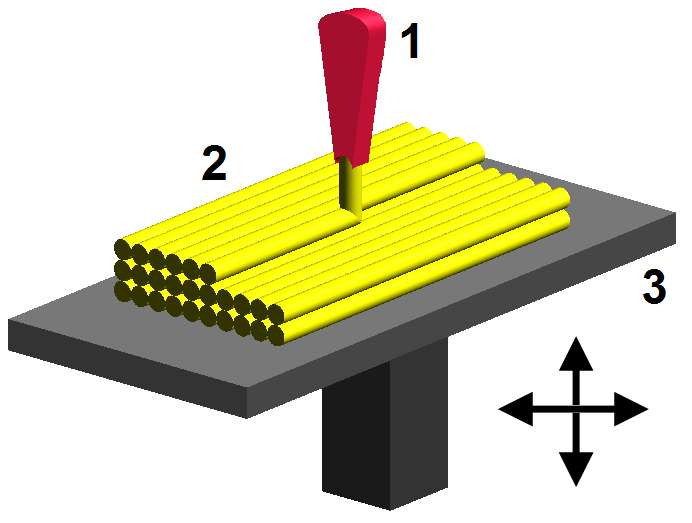
\includegraphics[width=0.4\textwidth]{images/FDM_by_Zureks.png}
            \caption{Principio de la fabricación con filamento fundido.}
            \label{fig:impr_fdm}
    \end{figure}

El principio de funcionamiento de este tipo de impresoras es la deposición de un material, en este caso un plástico fundido, en distintas capas. La máquina dispone de un elemento fusor, que está por encima de la temperatura de fusión del polímero, haciendo que entre en un estado viscoso y maleable. El fusor a su vez es capaz de desplazarse en los tres ejes cartesianos (X,Y,Z) a la vez que va depositando el polímero fundido. De este modo, la pieza es creada con el filamento que solidifica al salir del fusor.

\subsection{Materiales usados en impresión 3D}
\label{impreso_materiales}
En la actualidad hay multitud de materiales que se pueden usar en las impresoras 3D. Siendo la mayoría de ellos polímeros termoplásticos, ya que si se les aplica una temperatura alta se vuelven deformables y al enfriarlos, pasando por un estado de transición vítrea, se endurecen.\\

Algunos materiales que se usan son:
\begin{itemize}
    \item \textbf{ABS} o acrilonitrilo butadieno estireno.
    \item \textbf{PLA} o poliácido láctico.
    \item \textbf{PVA} o alcohol de polivinilo.
    \item \textbf{NYLON.}
\end{itemize}

Todos ellos tienen características que hacen idóneo su uso en diferentes campos. Por ejemplo, el ABS tiene unas propiedades mecánicas mejores que el PLA. Por ello, en función de la utilidad que se vaya a dar a la pieza final, será recomendable usar un polímero u otro. Todos estos consumibles comparten la característica de como se distribuyen. El polímero es introducido en el fusor de la impresora en forma de filamento para de ese modo conseguir un hilo continuo durante la impresión.\\

Por ello, el método de fabricación del consumible es la extrusión, ya que es el método que mejor se amolda para crear objetos con una sección transversal definida y fija.

\section{Extrusión de polímeros}
\label{arte_extrusion}
La extrusión de polímeros es un proceso industrial de fabricación, en el cual  se hace pasar por un troquel (también denominado dado) la matería prima previamente prensada y calentada. El proceso de prensado y calentamiento, se hace en una cámara, que contiene un tornillo sin fin el cual gira concentricamente y es alimentado por una tolva. Al hacer pasar el polímero por el troquel, se consigue un objeto con un perfil constante y una longitud variable, pudiendo llegar a ser de centímetros, o en algunos casos de metros.\footnote{ \url{http://es.wikipedia.org/wiki/Extrusi%C3%B3n_de_pol%C3%ADmero} }\\ 

\begin{figure}[H]
        \centering
        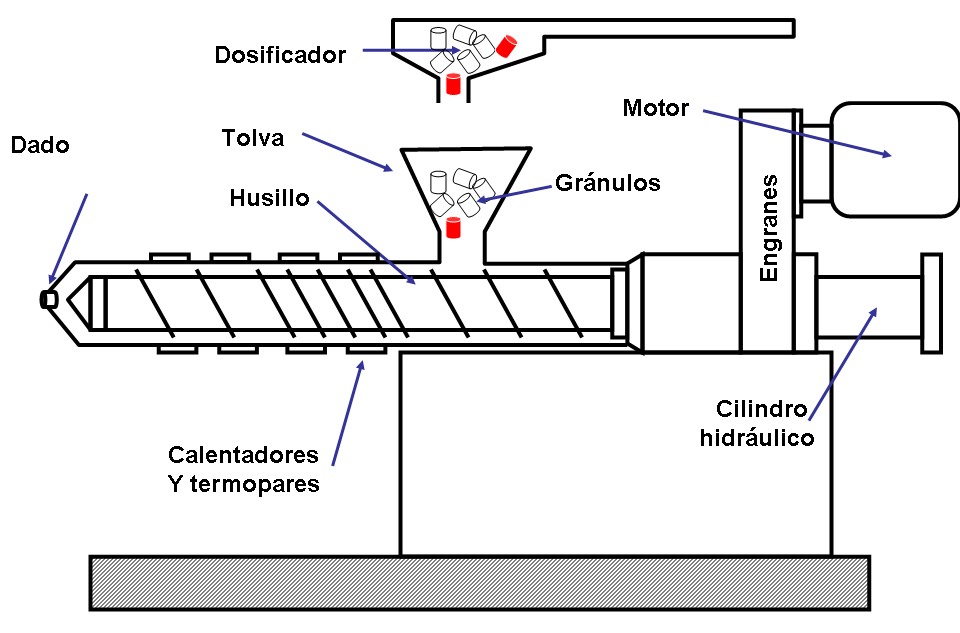
\includegraphics[width=0.6\textwidth]{images/extrusor.png}
        \caption{Esquema básico de una extrusora}
        \label{fig:estado_extrusora}
\end{figure}

Las principales variables de control que inluyen en el acabado del producto final, son la velocidad de extrusión y la temperatura del cilindro hidráulico afectando estos en la calidad final del producto.\\

La velocidad influye directamente en el caudal de producción de la máquina. Teóricamente, al incrementar la velocidad del husillo, obtendríamos una mayor producción en la línea, por contra repercute en la calidad final haciendo que la mezcla del producto no sea homogena y llegando a producirse la denominada fractura del polímero fundido, que es debido a la fricción que sufre el polímero al salir por el dado.\\

La temperatura por contra, influye en la viscosidad del polímero, este parámetro repercute directamente en la resistencia al fundido. Lo cual es bastante importante, por que en el caso que nos ocupa, el  material obtenido será posteriormente fundido en una impresora 3D.\\

Los distintos elementos que conforman la extrusora son los siguientes.
\begin{itemize}
    \item \textbf{Dosificador:} es el encargado de suministrar el polímero, normalmente en forma de granza, a la tolva garantizando un suministro constante.
    \item \textbf{Tolva:} despósito en el que cae la granza proveniente del dosificador. Debe proveer un flujo constante al extrusor para evitar cortes en el objeto que se está construyendo. Su diseño es muy importante, y en función del tipo de material que esté suministrando deberá ser de una manera u otra, debido a que el material puede llegar a compactarse en el fondo y no pasar a la extrusora. Algunos modelos de tolva incluyen sistemas de vibración para ayudar a que el material caiga. En la mayoría de los casos y dependiendo del material con el que estemos trabajando, será conveniente que incluya un sistema de secado para eliminar la humedad, puesto que puede afectar a la hora de trabajar con el.
    \item \textbf{Cilindro hidráulico:} Constituye el cuerpo principal de la extrusora y en su interior está el husillo. Es en este cilindro donde se encuentran las resistencias electricas que aportan la energía calorífica necesaria para fundir el material. La temperatura está registrada a lo largo de las distintas zonas del cilindro, para poder tener un control sobre la temperatura de fusión del material. El cilindro debe estar fabricado con materiales especiales de tal manera, que tenga una buena transferencia de calor y debe ser más duro que el materíal que se está extruyendo, para lograr una larga duración.
    \item \textbf{Husillo:} Es el elemento más importante de la extrusora y el que determina el grado de calidad con el que la pieza saldrá de la extrusora.\\
            \begin{figure}[H]
                      \centering
                        \begin{subfigure}[b]{0.55\textwidth}
                                \centering
                            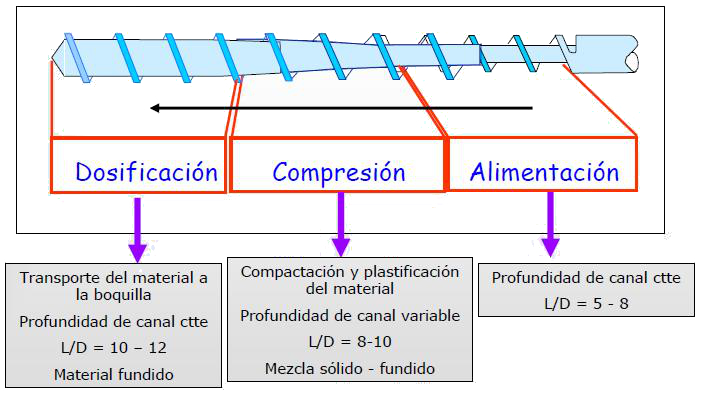
\includegraphics[width=\textwidth]{images/husillo.jpg}
                            \caption{Forma de un husillo.}
                            \label{fig:estado_husillo1}
                        \end{subfigure}
                        
                        \begin{subfigure}[b]{0.55\textwidth}
                                \centering
                            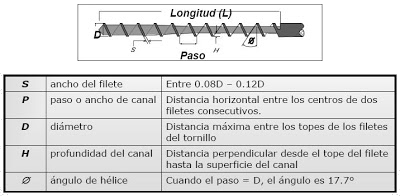
\includegraphics[width=\textwidth]{images/husillo2.jpg}
                            \caption{Parámetros de un husillo.}
                            \label{fig:estado_husillo2}
                        \end{subfigure}
                        \caption{Características de un husillo.}
                        \label{fig:estado_husillo}
            \end{figure}
    Como se aprecia en la figura \ref{fig:estado_husillo1} tenemos tres zonas claramente definidas:
    \begin{itemize}
            \item \textbf{Alimentación:} Esta zona, es la encargada de transportar la granza de la tolva al interior del husillo. En la figura \ref{fig:estado_husillo1} podemos ver como los filetes están muy separados del centro del husillo, con el fin de transportar la mayor cantidad posible de material.
            \item \textbf{Compresión:} A medida que entramos en la zona de compresión, los filetes van disminuyendo y se acercan al husillo, con el fin de fundir y homogeneizar el material. Aquí se expulsa el posible aire residual que quede entre la granza.
            \item \textbf{Dosificación:} Conduce el material compactado hacia el dado de la extrusora. Esta zona debe garantizar que el material sale con una temperatura constante y homogeneo.
    \end{itemize}
    \item \textbf{Dado:} En función del dado que se coloque al final de la extrusora, se conseguirá un perfil distinto, en el caso que nos ocupa, el dado tiene un círculo para conseguir la forma de cilindro que deseamos.
    \begin{figure}[H]
            \centering
            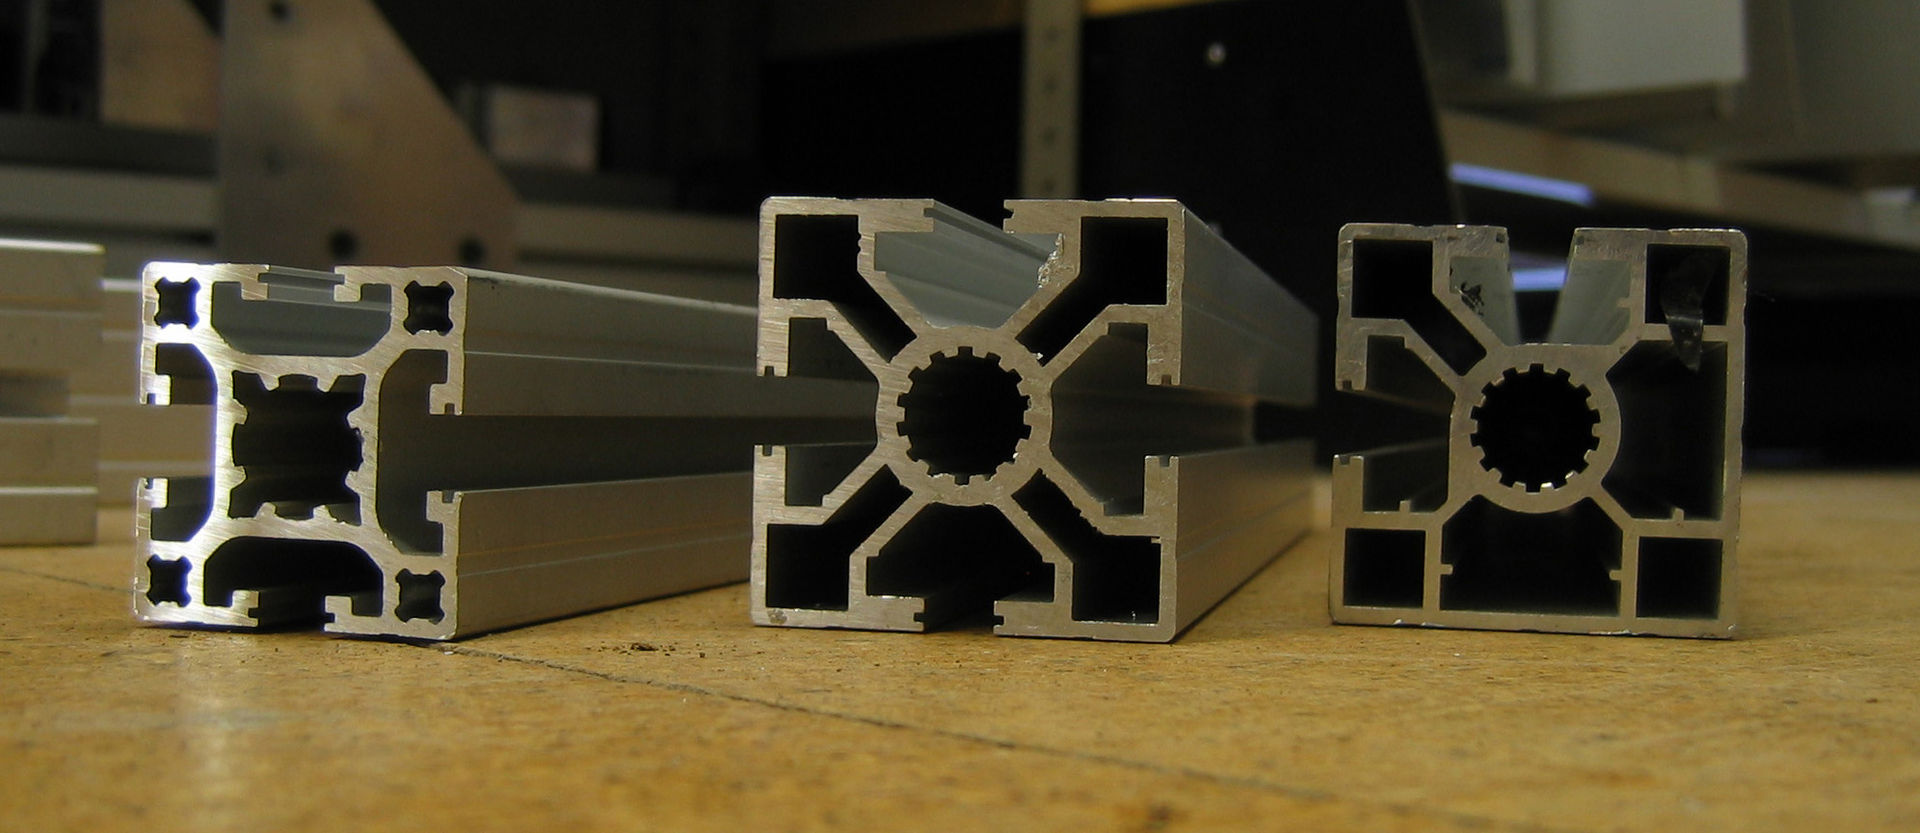
\includegraphics[width=0.5\textwidth]{images/Extruded_aluminium_section.jpg}
            \caption{Distintos ejemplos de extrusión.}
            \label{fig:estado_ejemplos}
    \end{figure}
\end{itemize}

\section{Fundamentos del control}
\label{arte_control}
\section{Comunicaciones industriales}
\label{arte_comunicaciones}

\subsection{Capas de comunicación}
\label{comunic_capas}
El modelo OSI establece en siete capas, cualquier proceso de transmisión entre equipos informáticos. Cada capa, tiene una tarea especifica en la que después de pasar por ella se va añadiendo una cabecera al paquete que posteriormente se enviará por el medio físico.
    \begin{figure}[H]
            \centering
            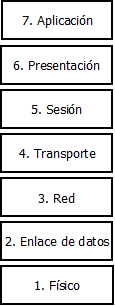
\includegraphics[width=0.1\textwidth]{images/capas_osi.png}
            \caption{Capas del modelo OSI.}
            \label{fig:capas_osi}
    \end{figure}
De esta manera se estandariza el uso de cualquier protocolo de comunicaciones que se vaya a usar. Cabe destacar, que tanto en el caso del emsior, como el receptor se usa el mismo modelo, pero en un caso se ejecuta de forma ascendente (de la capa 1 a la 7) y en el otro de forma descendente (de la capa 7 a la 1).
\subsection{Profibus}
\label{comunic_profibus}
Es un estandar de comunicaciones para buses de campo desarrollado por la empresa Siemens. Al igual que otros protocolos, como MODBUS, se puede esablecer el enlace físico entre los dispositivos de la red, mediante diferentes tecnologías:
\begin{itemize}
    \item TCP/IP sobre Ethernet.
    \item Transmisión serie asíncrona(RS-232,RS-485,fibra óptica,etc)
\end{itemize}
Según la aplicación que se vaya a desarrollar, hay distintos protocolos de profibus que ofrecen ventajas específicas en cada caso.
\begin{itemize}
    \item \textbf{Profibus-DP (Descentralized Periphery):} Específico para comunicacion entre un sistema de control y entradas/salidas distribuidas por la fábrica(campo).
    \item \textbf{Profibus-PA (Processs Automation):} Permite que sensores y actuadores sean conectados al bus. Suele estár orientado a un ámbido de seguridad.
    \item \textbf{Profibus-FMS (Field Message Specification):} Permite la coordinacion de las distintas aplicaciones de comunicación que puede haber en la industría: Buses de ordenadores industriales, robots,...
\end{itemize}
    \begin{figure}[H]
            \centering
            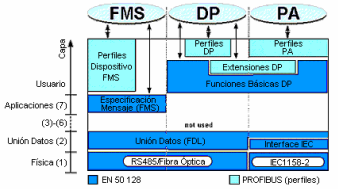
\includegraphics[width=0.5\textwidth]{images/protocolo_profibus.png}
            \caption{Protocolo de comunicaciones de profibus.}
            \label{fig:protocolo_profibus}
    \end{figure}
Profibus establece al menos un maestro (normalmente un PLC) y varios esclavos (periferia descentralizada,sensores, actuadores,...) dentro del bus. De esta manera, el maestro manda mensajes a los esclavos los cuales, responderan. El mensaje o trama que se manda puede tener hasta 3 formatos:
\begin{itemize}
    \item trama de longitud fija sin datos.
    \item trama de longitud fija con datos.
    \item trama de longitud variable.
\end{itemize}

\subsection{MODBUS}
\label{comunic_modbus}
El MODBUS es un protocolo de comunicaciones que se situa en el nivel 7 del modelo de comunicaciones OSI (Visto en capítulo \ref{comunic_capas}). El cual facilita la comunicacion entre cliente/servidor conectados mediante distintos tipos de buses de comunicación commo pueden ser:

\begin{itemize}
    \item TCP/IP sobre Ethernet.
    \item Transmisión serie asíncrona(RS-232,RS-485,fibra óptica,etc)
\end{itemize}

El protocolo define una unidad de dato simple (\textbf{PDU}), el cual es independiente del tipo de bus de comunicación usado. Y en función de la comunicación usada, la unidad de dato de aplicación (\textbf{ADU}) tendrá un tipo de información distinta (Ver imagen \ref{fig:paquete_modbus}).
    \begin{figure}[H]
            \centering
            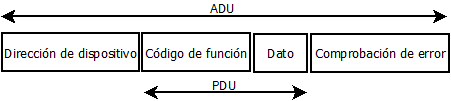
\includegraphics[width=0.5\textwidth]{images/trama_modbus.png}
            \caption{Detalle de un paquete de MODBUS.}
            \label{fig:paquete_modbus}
    \end{figure}
Cada parte del paquete incluye la siguiente información:
\begin{itemize}
    \item \textbf{Dirección de dispositivo:} Incluye la dirección del dispositivo sobre el que se va a ejecutar el código de función.
    \item \textbf{Código de función:} Dentro de la trama ocupa un byte y puede contener cualquier valor desde 1 a 255 el cual indicará una función a ejecutar por parte del servidor o cliente (Ver tabla \ref{tab:funcion_modbus}).
    \item \textbf{Dato:} Contiene la información que devuelve el cliente al servidor, el cual se usará para realizar la acción definida en el código de función. Este campo puede estar vacio o contener el número de elementos con los que se quiere trabajar.
    \item \textbf{Comprobación de error:} En caso de ocurrir algún error relacionado con el código de función, se añadirá un código de error en este campo, que el servidor deberá de procesar para determinar qué acción ejecutar.
\end{itemize}
\begin{table}[!hbt]
  \centering
  \begin{tabular}{|c|c|c|}
    \hline
    Descripción & código decimal & código hexadecimal\\
    \hline
    Read Discrete Inputs & 02  & 02\\
    \hline
    Read Coils & 01  & 02\\
    \hline
    Write Single Coil & 05  & 05\\
    \hline
    Write Multiple Coils & 15  & 0F\\
    \hline
    Read Input Register & 04  & 04\\
    \hline
    Read Holding Registers & 03  & 03\\
    \hline
    Write single Register & 06  & 06\\
    \hline
    Write Multiple Registers & 16  & 10\\
    \hline
  \end{tabular}
  \caption{Tabla obtenida del protocol de MODBUS.}
  \label{tab:funcion_modbus}
\end{table}
A continuación se detalla un ejemplo de petición de un servidor hacía un cliente para leer tres registros análógicos. El paquete a mandar por el servidor será:\\
\begin{center}
    \textit{11 03 006B 0003 7687}
\end{center}
\begin{itemize}
    \item \textbf{11} Dirección del esclavo (0x11=17)
    \item \textbf{03} Código de función. (Ver tabla \ref{tab:funcion_modbus}).
    \item \textbf{006B} Dirección en hexadecimal donde se encuentra el primer registro.
    \item \textbf{0003} Número total de registros que se quieren leer. Del 40108 al 40110.
    \item \textbf{7687} Código CRC para la comprobación de errores.
\end{itemize}
A lo que el esclavo responderá un paquete similar a este:\\
\begin{center}
    \textit{11 03 06 AE41 5652 4340 49AD}
\end{center}
\begin{itemize}
    \item \textbf{11} Dirección del esclavo (0x11=17)
    \item \textbf{03} Código de función. (Ver tabla \ref{tab:funcion_modbus}).
    \item \textbf{06} Dirección en hexadecimal donde se encuentra el primer registro.
    \item \textbf{AE41} Contenido del registro 40108
    \item \textbf{5652} Contenido del registro 40109
    \item \textbf{4340} Contenido del registro 40110
    \item \textbf{49AD} Código CRC para la comprobación de errores.
\end{itemize}

\subsection{Device Net}
\label{comunic_device}



\subsection{AS-I}
\label{comunic_asi}
Es un bus de comunicaciones de campo para interconectar sensores y actuadores con el maestro de la red, normalmente un PLC. Por ello, se situa en la parte má baja de la piramide de comunicaciones, situandose directamente en campo.\\

El maestro de AS-i se encarga de mirar uno a uno el estado de los sensores(polling). Una fuente de alimentación especial, se encarga de llevar la alimentación a cada uno de los sensores a la vez que la información de cada uno al maestro. De esta manera, con únicamente dos cables se establece la comunicación.\\



